\documentclass{article}

% Formatting
\usepackage[utf8]{inputenc}
\usepackage[margin=1in]{geometry}
\usepackage[titletoc,title]{appendix}
\usepackage[spanish]{babel}
\usepackage{amsmath,amsfonts,amssymb,mathtools}
\usepackage{graphicx,float}
\usepackage[ruled,vlined]{algorithm2e}
\usepackage{algorithmic}
\usepackage{minted}
\usemintedstyle{borland}
\usepackage{subcaption}
\usepackage{multicol}
\usepackage{listings}
\usepackage{xcolor}
\usepackage{biblatex}
\addbibresource{ref.bib}
\usepackage{minted}



% Title content
\title{Práctica 9 interacciones entre partículas}
\author{Denisse Leyva}
\date{Abril 28, 2021}

\begin{document}

\maketitle


\section{Introducción}
En esta práctica trabajaremos con un modelo simplificado para los fenómenos de atracción y repulsión de física (o química de hecho). Supongamos que contamos con $n$ partículas que habitan un cuadro unitario bidimensional y que cada partícula tiene una carga eléctrica, distribuida independiente y normalmente al azar entre $[-1, 1]$. Cargas de un mismo signo producirán una repulsión mientras cargas opuestas resultan en una atracción, la magnitud de la fuerza estará proporcional a la diferencia de magnitud de las cargas (mayores diferencias resultando en fuerzas mayores), y además la fuerza será inversamente proporcional a la distancia euclidiana entre las partículas \cite{Satu_Elisa_Schaeffer}.

\section{Objetivo}
Agregar a cada partícula una masa y haz que la masa cause fuerzas gravitacionales (atracciones) además de las fuerzas causadas por las cargas. Estudia la distribución de velocidades de las partículas y verifica gráficamente que esté presente una relación entre los tres factores: la velocidad, la magnitud de la carga, y la masa de las partículas. Toma en cuenta que la velocidad también es afectada por las posiciones \cite{Satu_Elisa_Schaeffer}. 

\section{Código}

Para realizar el código base se determinó una constante gravitacional definida por mí y se usó la fórmula de la fuerza gravitacional. Para obtener la fuerza total se sumaron las fuerzas generadas por las cargas y las fuerzas generadas por la masa. El código base se sacó de Schaeffer \cite{Elisa_Schaeffer}. El código completo se encuentra en el GitHub \cite{Denisse_Leyva}.

\renewcommand{\listingscaption}{Código}
\begin{listing}[H]
  \begin{minted}[linenos,mathescape,texcl]{clojure}
  G = 0.001 #Suponemos que la constante gravitacional es 0.001
def fuerza(i, shared):
    p = shared.data
    n = shared.count
    pi = p.iloc[i]
    xi = pi.x
    yi = pi.y
    ci = pi.c
    mi = pi.m
    fx1, fy1 = 0, 0
    fx2, fy2 = 0, 0
    for j in range(n):
        pj = p.iloc[j]
        cj = pj.c
        mj = pj.m
        dire = (-1)**(1 + (ci * cj < 0))
        dx = xi - pj.x
        dy = yi - pj.y
        factor = dire * fabs(ci - cj) / (sqrt(dx**2 + dy**2) + eps)
        factor1 = G * (((mi * mj) / ((sqrt(dx**2 + dy**2) + eps)**2)))
        fx1 = fx1 - dx * factor
        fy1 = fy1 - dy * factor
        fx2 = fx2 - dx * factor1
        fy2 = fy2 - dy * factor1
    
    fx = fx1 + fx2
    fy = fy1 + fy2
    return (fx, fy)
      \end{minted}
  \label{lst:fibo}
  \caption{Sumatoria de fuerzas.}
\end{listing}

\renewcommand{\listingscaption}{Código}
\begin{listing}[H]
  \begin{minted}[linenos,mathescape,texcl]{clojure}
def velocidad(p, pa):
    ppa = pa.data
    n = pa.count
    for i in range(n):
      p1 = p.iloc[i]
      p2 = ppa.iloc[i]
      x1 = p1.x
      x2 = p2.x
      y1 = p1.y
      y2 = p2.y
      va = p2.v
      v = []
      v.extend(va)
      vel = (sqrt(((x2 - x1)**2) + ((y2 - y1)**2)))
      v.append(vel)
      p['v'][i] = v
      \end{minted}
  \label{lst:fibo}
  \caption{Obtener velocidad resultante por iteración.}
\end{listing}

\section{Resultados}

En las gráficas se observa un cambio cuando actúan las fuerzas de la masa y la carga en comparación cuando actúa solo la carga.  También se nota que dependiendo de la fuerza que se aplique es la velocidad que toma la partícula. En el GitHub se encuentran los gif \cite{Denisse_Leyva}.

\begin{figure}[H]
\centering
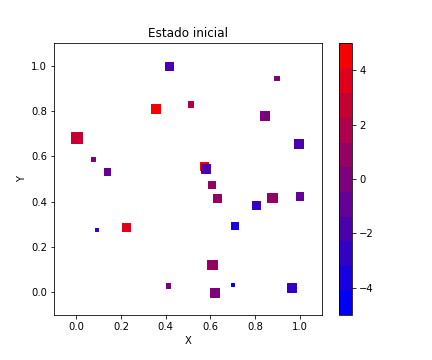
\includegraphics[width=80mm]{p9pc_t0.png}
\caption{\label{fig3} Estado Inicial.}
\end{figure}

\begin{figure}[H]
\centering
\begin{subfigure}[b]{0.40\linewidth}
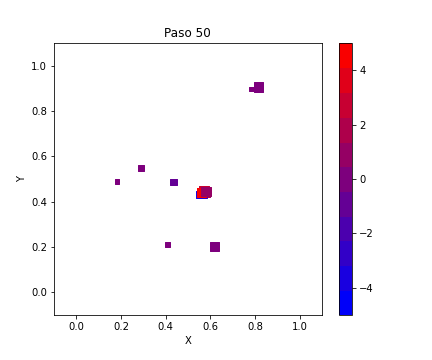
\includegraphics[width=\linewidth]{p9pc_t50.png}
\caption{Estado final usando como fuerza la carga de la partícula.}
\end{subfigure}
\begin{subfigure}[b]{0.40\linewidth}
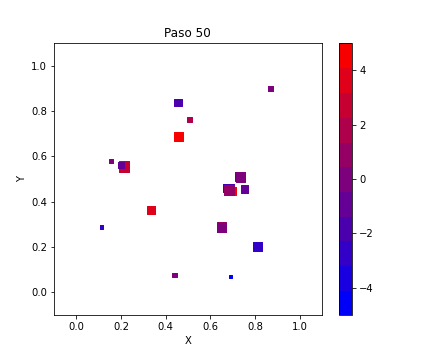
\includegraphics[width=\linewidth]{p9pm_t50.png}
\caption{Estado final usando como fuerza la masa de la partícula.}
\end{subfigure}
\caption{Imagénes de estado final con diferentes fuerzas.}
\label{fig:westminster}
\end{figure}


\begin{figure}[H]
\centering
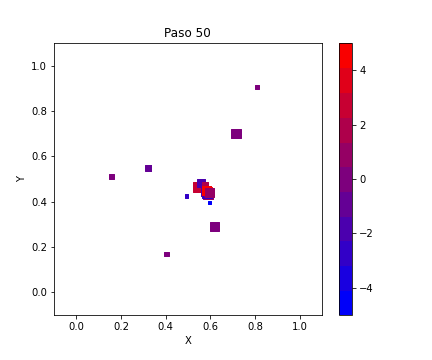
\includegraphics[width=80mm]{p9pmc_t50.png}
\caption{\label{fig3} Estado final usando las fuerzas de la masa y la carga de la partícula.}
\end{figure}

\begin{figure}[H]
\centering
\begin{subfigure}[b]{0.40\linewidth}
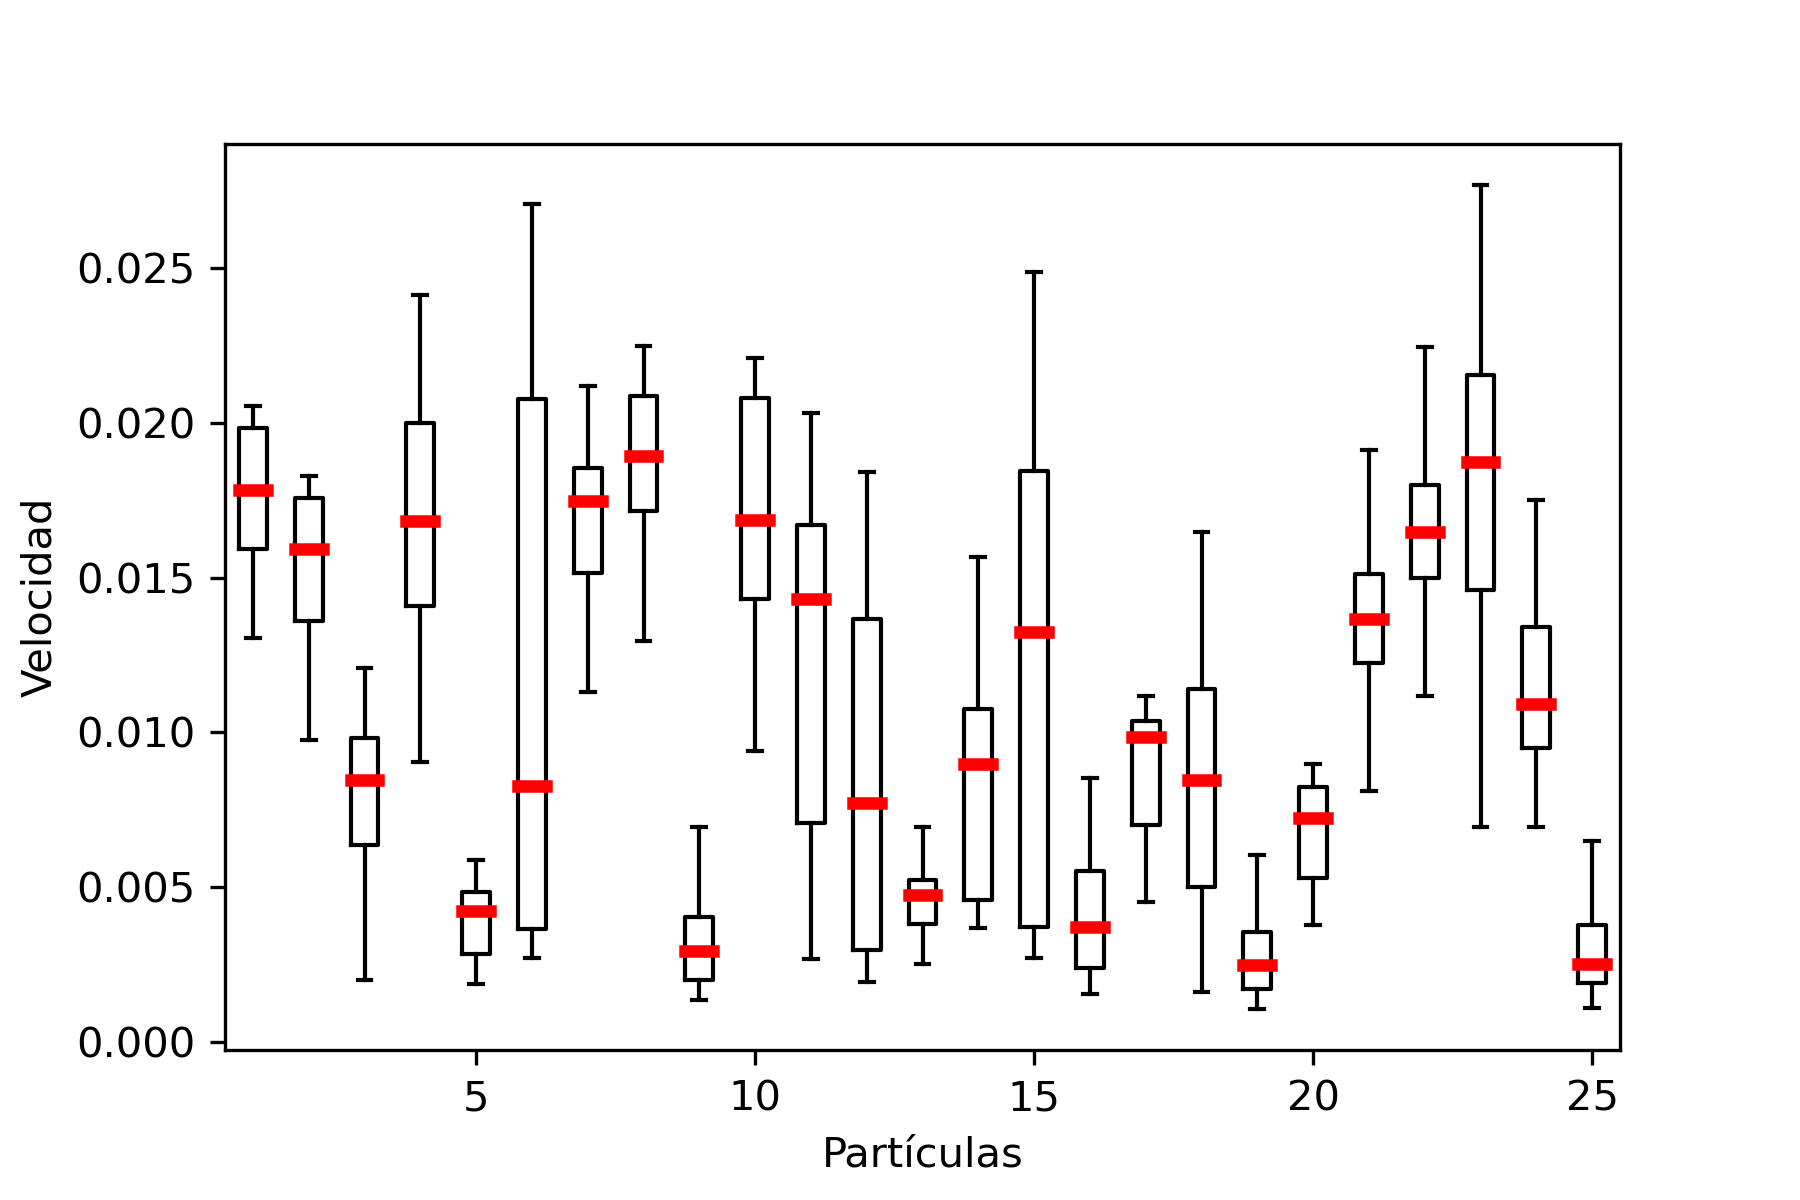
\includegraphics[width=\linewidth]{p9pc.png}
\caption{Gráfica de velocidad aplicando solo la fuerza de la carga.}
\end{subfigure}
\begin{subfigure}[b]{0.40\linewidth}
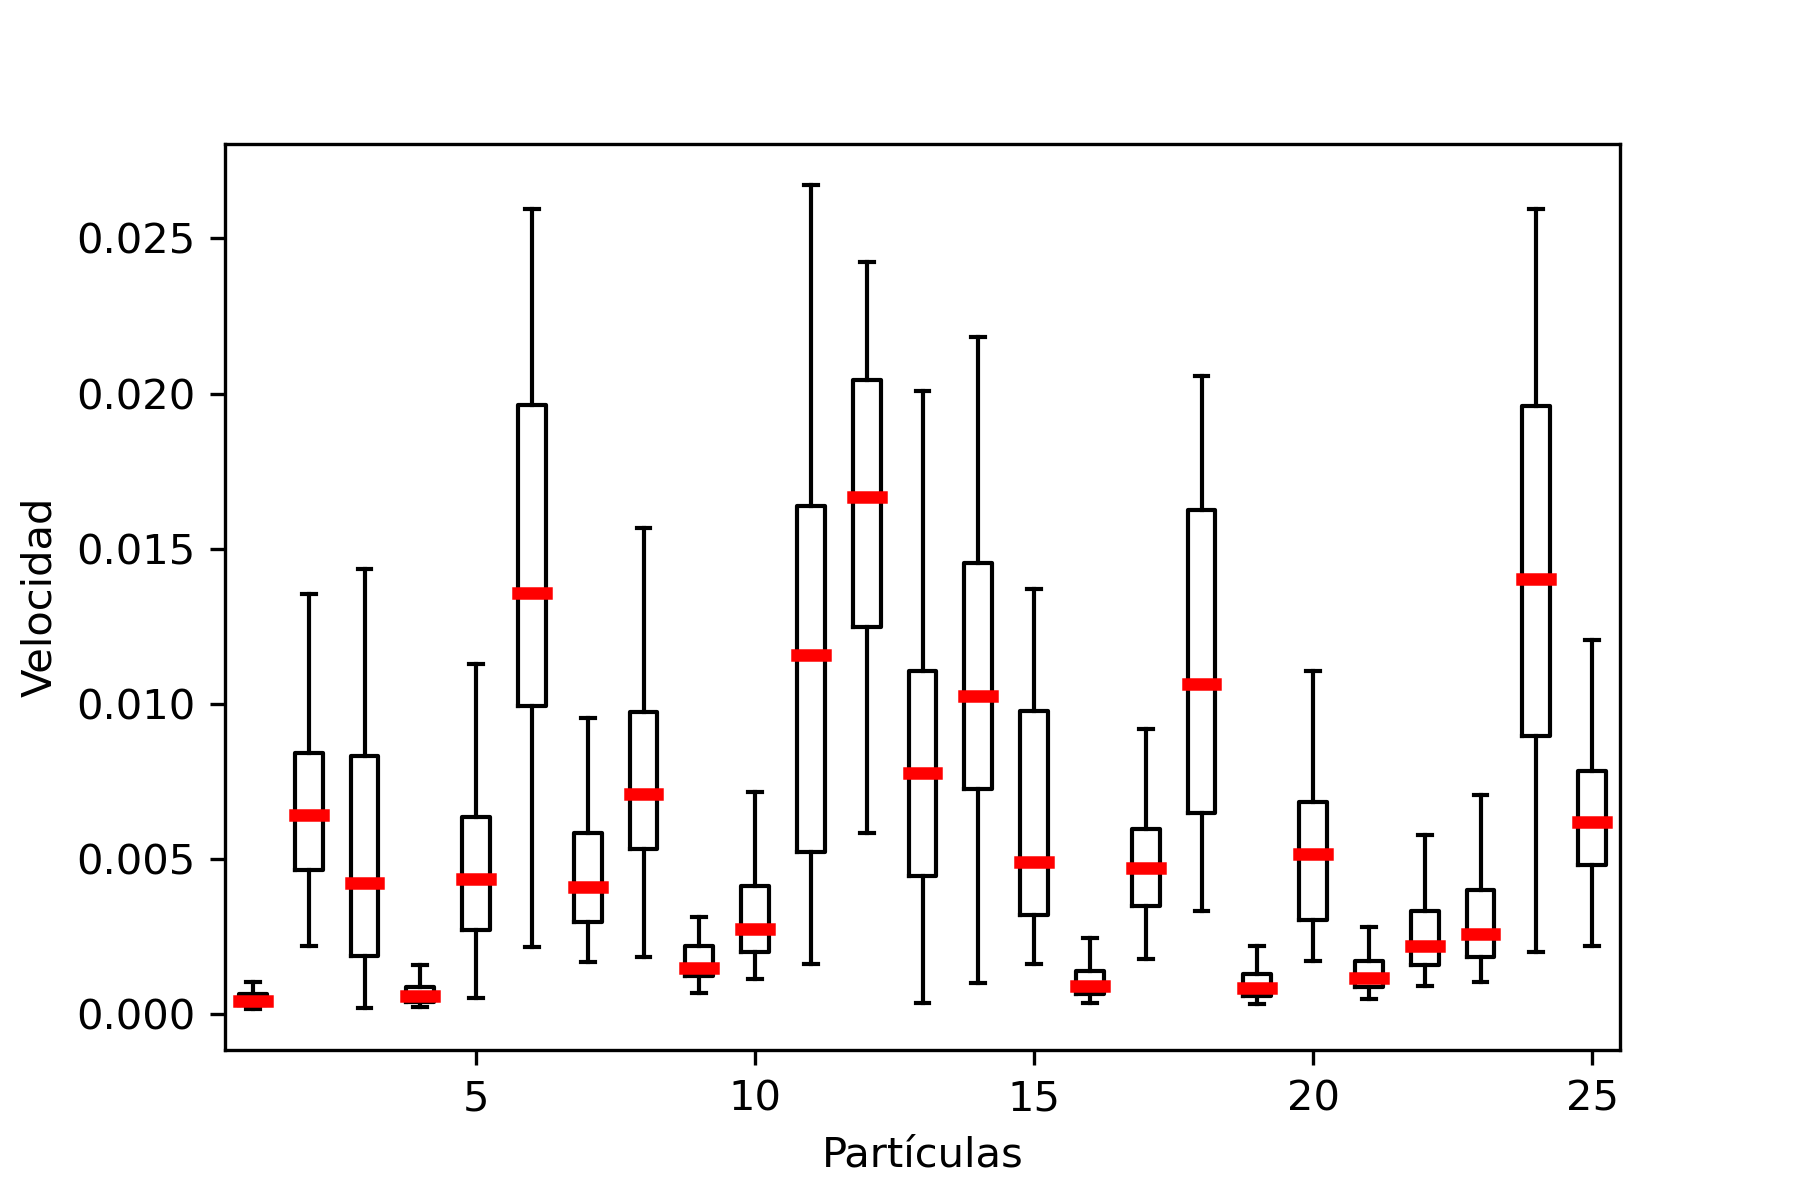
\includegraphics[width=\linewidth]{p9pm.png}
\caption{Gráfica de velocidad aplicando solo la fuerza de la masa.}
\end{subfigure}
\caption{Gráficas de velocidad con diferentes fuerzas por partícula.}
\label{fig:westminster}
\end{figure}

\begin{figure}[H]
\centering
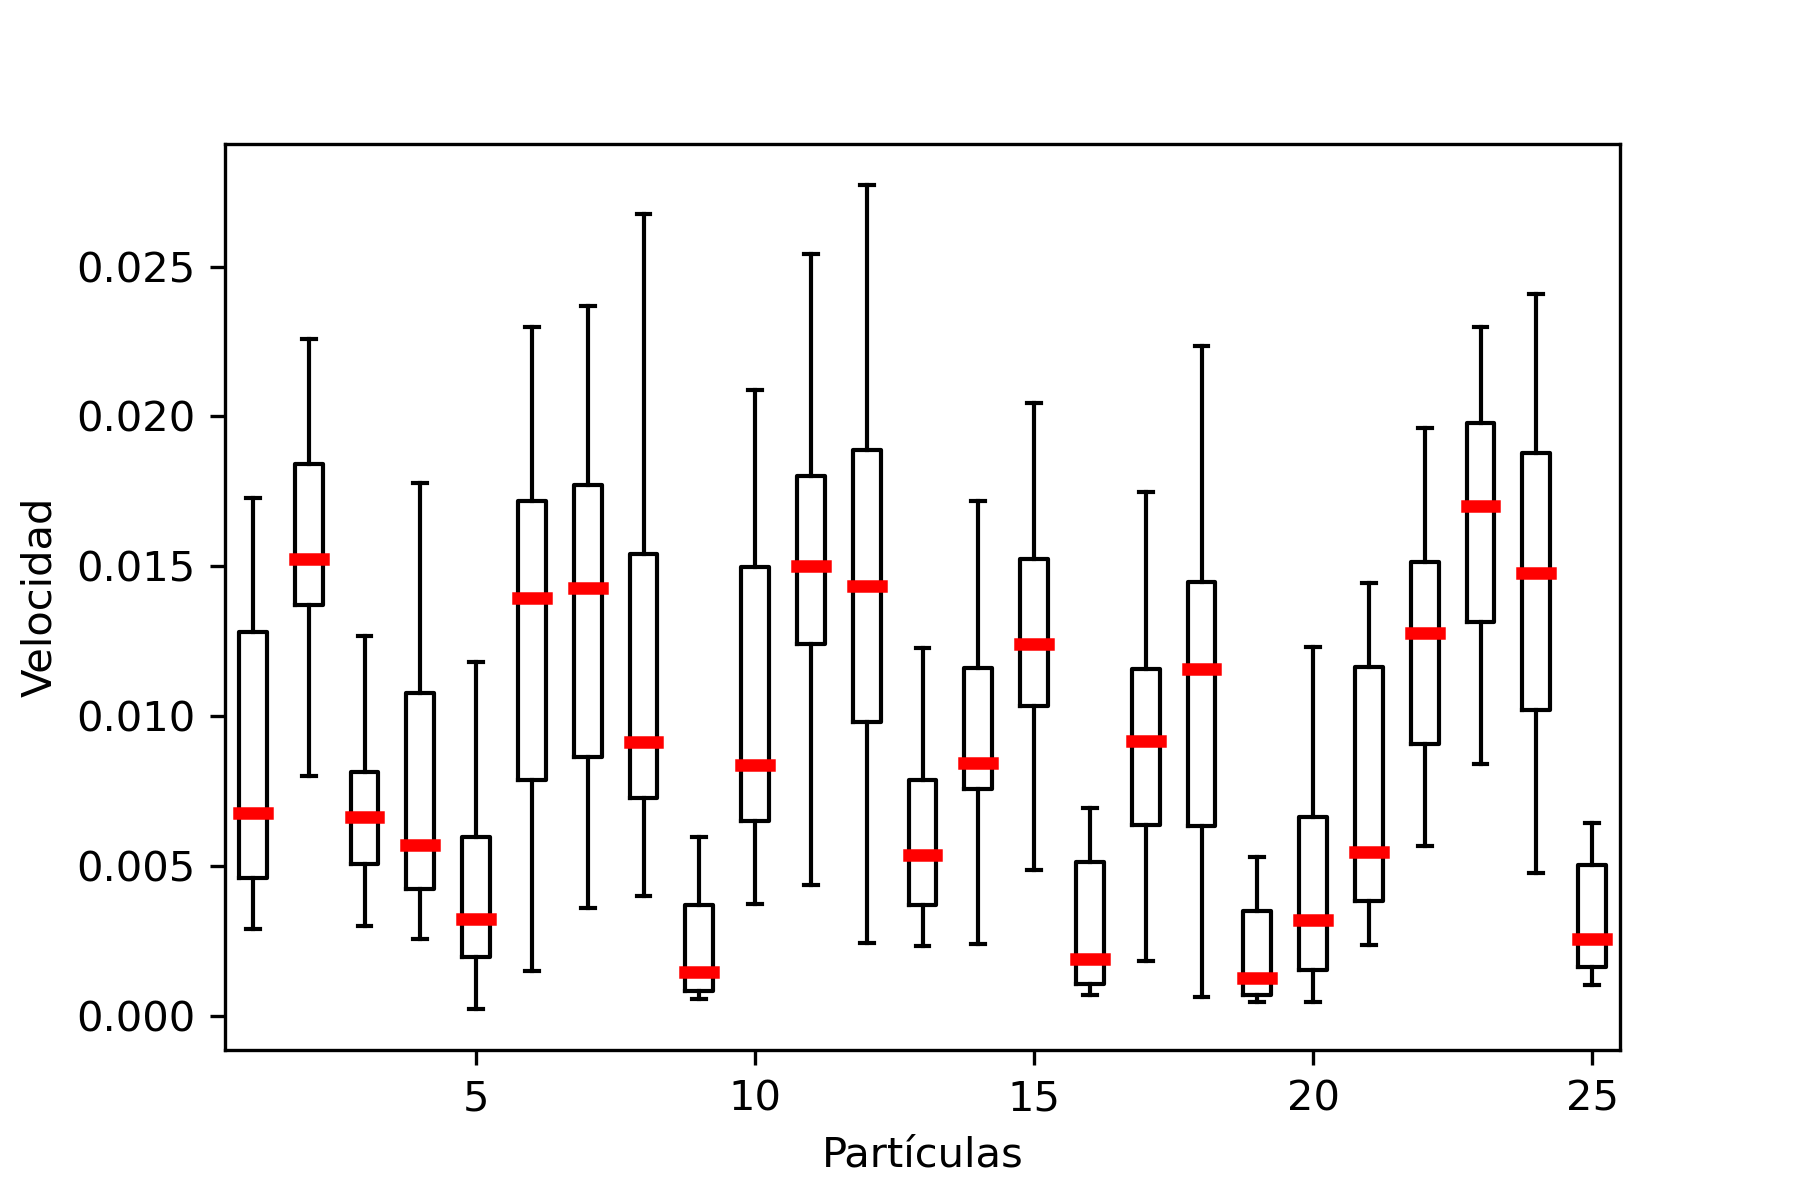
\includegraphics[width=80mm]{p9pmc.png}
\caption{\label{fig3} Gráfica de velocidad aplicando las fuerza de la carga y la masa.}
\end{figure}

\section{Reto 1}
El primer reto es simular dos diferentes tipos de objetos: bolitas duras grandes y partículas frágiles, cuando una partícula es atrapada entre dos bolas, se modifica: si está sola, se fragmenta, pero si hay otras partículas en esa misma traslape de dos bolas, se pegan todos juntos. Haz que las bolitas y las partículas reboten de los bordes de la zona \cite{Satu_Elisa_Schaeffer}.

Para las reglas primero se generó un ciclo for para ir de partícula en partícula, dentro de ese for se generó otro for para determinar las distancias euclidianas de esa partícula referente a las bolas. Si la distancia es menor a la distancia total de los radios de la partícula y la bola se genera un conteo así cuando el conteo llega a dos se sabrá que hay dos bolas sobre esa partícula. Luego de esto continua la parte de unir y romper partículas mostrada en los siguientes códigos.

\renewcommand{\listingscaption}{Código}
\begin{listing}[H]
  \begin{minted}[linenos,mathescape,texcl]{clojure}
for i in range(m):
        b = bolas.iloc[i]
        br = b.r
        bx = b.x
        by = b.y
        vx = b.dx
        vy = b.dy
        x = bx + vx
        y = by + vy
        if 0 >= (x-br):
            x = 0 + br
            bolas.at[i, 'dx'] = vx * -1
        elif (x+br) >= 1:
            x = 1 - br
            bolas.at[i, 'dx'] = vx * -1
        if 0 >= (y-br):
            y = 0 + br
            bolas.at[i, 'dy'] = vy * -1
        elif (y+br) >= 1:
            y = 1 - br
            bolas.at[i, 'dy'] = vy * -1
        
        bolas.at[i, 'x'] = x
        bolas.at[i, 'y'] = y
      \end{minted}
  \label{lst:fibo}
  \caption{Genera el movimiento de las bolas.}
\end{listing}

\renewcommand{\listingscaption}{Código}
\begin{listing}[H]
  \begin{minted}[linenos,mathescape,texcl]{clojure}
for i in range(n):
        b = particulas.iloc[i]
        br = b.r
        bx = b.x
        by = b.y
        vx = b.dx
        vy = b.dy
        x = bx + vx
        y = by + vy
        if 0 >= (x-br):
            x = 0 + br
            particulas.at[i, 'dx'] = vx * -1
        elif (x+br) >= 1:
            x = 1 - br
            particulas.at[i, 'dx'] = vx * -1
        if 0 >= (y-br):
            y = 0 + br
            particulas.at[i, 'dy'] = vy * -1
        elif (y+br) >= 1:
            y = 1 - br
            particulas.at[i, 'dy'] = vy * -1
        
        particulas.at[i, 'x'] = x
        particulas.at[i, 'y'] = y
      \end{minted}
  \label{lst:fibo}
  \caption{Genera el movimiento de las partículas.}
\end{listing}


\renewcommand{\listingscaption}{Código}
\begin{listing}[H]
  \begin{minted}[linenos,mathescape,texcl]{clojure}
for j in range(n):
    if i != j:
        pj = particulas.iloc[j]
        pjr = pj.r
        pjx = pj.x
        pjy = pj.y
        dx = px - pjx
        dy = py - pjy
        dr = pjr + pr
        d = sqrt(dx**2 + dy**2)
        if d < dr: # Unir particulas
            conteo2 += 1
            a1 = np.pi * (pr**2)
            a2 = np.pi * (pjr**2)
            a = a1 + a2
            rt = sqrt(a/np.pi)
            particulas.at[i, 'r'] = rt
            particulas.at[j, 'v'] = -1
      \end{minted}
  \label{lst:fibo}
  \caption{Une partículas.}
\end{listing}

\renewcommand{\listingscaption}{Código}
\begin{listing}[H]
  \begin{minted}[linenos,mathescape,texcl]{clojure}
if conteo2 == 0: # Romper particulas
    v = random()
    v1 = 1 - v
    vx1 = p.dx * -1
    vy1 = p.dy * -1
    a = np.pi * (pr**2)
    a1 = a * v
    a2 = a * v1
    r1 = sqrt(a1/np.pi)
    r2 = sqrt(a2/np.pi)
    particulas.at[i, 'r'] = r1
    particulas = particulas.append({'x': px, 'y': py, 'dx': vx1, 'dy': vy1, 
                                    'r': r2, 'v': 1, 'a': 1}, ignore_index=True)
      \end{minted}
  \label{lst:fibo}
  \caption{Separa partículas.}
\end{listing}



\printbibliography
\end{document}
